\begin{figure}[h]
  \centering
  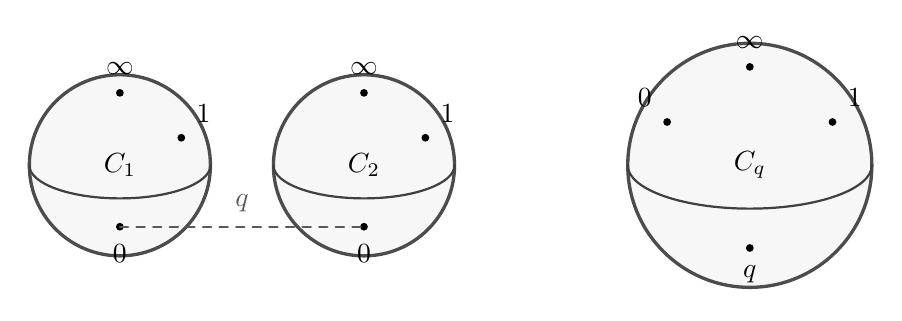
\begin{tikzpicture}[scale=1.0, line cap=round, line join=round]
    % parameters
    \def\R{1.15}

    % left thrice-marked sphere
    \begin{scope}[shift={(-4.1,0)}]
      \fill[gray!6] (0,0) circle (\R);
      \draw[very thick, gray!60!black] (0,0) circle (\R);
      \draw[gray!50!black, thick] (-\R,0) arc (180:360:{\R} and {0.42});

      \coordinate (L0) at (0,-0.78);
      \coordinate (L1) at (0.78,0.35);
      \coordinate (Linf) at (0,0.92);

      \fill[black] (L0) circle (1.4pt);
      \fill[black] (L1) circle (1.4pt);
      \fill[black] (Linf) circle (1.4pt);

      \node[below=3pt] at (L0) {$0$};
      \node[above right=2pt] at (L1) {$1$};
      \node[above=3pt] at (Linf) {$\infty$};

      \node at (0,0) {$C_1$};
    \end{scope}

    % right thrice-marked sphere
    \begin{scope}[shift={(-1.0,0)}]
      \fill[gray!6] (0,0) circle (\R);
      \draw[very thick, gray!60!black] (0,0) circle (\R);
      \draw[gray!50!black, thick] (-\R,0) arc (180:360:{\R} and {0.42});

      \coordinate (R0) at (0,-0.78);
      \coordinate (R1) at (0.78,0.35);
      \coordinate (Rinf) at (0,0.92);

      \fill[black] (R0) circle (1.4pt);
      \fill[black] (R1) circle (1.4pt);
      \fill[black] (Rinf) circle (1.4pt);

      \node[below=3pt] at (R0) {$0$};
      \node[above right=2pt] at (R1) {$1$};
      \node[above=3pt] at (Rinf) {$\infty$};

      \node at (0,0) {$C_2$};
    \end{scope}

    % dashed line connecting punctures to be plumbed
    \draw[thick, dashed, gray!70!black] (-4.1,-0.78) -- (-1.0,-0.78);
    \node[above=2pt, gray!70!black] at (-2.55,-0.78) {$q$};

    % sphere with four marked points; cross-ratio parameter q
    \begin{scope}[shift={(3.9,0)}]
      \def\RR{1.55}
      \fill[gray!6] (0,0) circle (\RR);
      \draw[very thick, gray!60!black] (0,0) circle (\RR);

      % equator
      \draw[gray!50!black, thick] (-\RR,0) arc (180:360:{\RR} and {0.55});

      % marked points (schematic positions)
      \coordinate (p0) at (-1.05,0.55);
      \coordinate (p1) at (1.05,0.55);
      \coordinate (pinf) at (0,1.25);
      \coordinate (pq) at (0,-1.05);

      \fill[black] (p0) circle (1.4pt);
      \fill[black] (p1) circle (1.4pt);
      \fill[black] (pinf) circle (1.4pt);
      \fill[black] (pq) circle (1.4pt);

      \node[above left=2pt] at (p0) {$0$};
      \node[above right=2pt] at (p1) {$1$};
      \node[above=3pt] at (pinf) {$\infty$};
      \node[below=3pt] at (pq) {$q$};

      \node at (0,0) {$C_q$};
    \end{scope}
  \end{tikzpicture}
  \caption{After plumbing two thrice-marked spheres at $0$ and $0$, the resulting sphere has four marked points with cross-ratio $q$.}
\end{figure}
